%! TEX root = /Users/circle/Documents/博二上/湍流/Turbulence/HW3/homework/homework.tex
\documentclass[12pt,a4]{ctexart}
\usepackage{natbib}
\usepackage{url}
\usepackage{stmaryrd}
\usepackage{mathrsfs}
\usepackage{amsmath}
\usepackage{graphicx}
\usepackage{parskip}
\usepackage{fancyhdr}
% \usepackage{underscore} % 下划线
\usepackage{commath}%定义d
\usepackage{geometry}
\usepackage{bm}
\usepackage{siunitx}
\usepackage{float}
% \usepackage[skip=-5pt]{subcaption}
% \usepackage{subfig}
\usepackage{subfigure}  %插入多图时用子图显示的宏包
\usepackage{titlesec}
\usepackage{caption}
\usepackage{paralist}
\usepackage{multirow}
\usepackage{booktabs} % To thicken table lines
\usepackage{diagbox}
\usepackage{authblk}
\usepackage{indentfirst}
\usepackage{amsthm}
\usepackage{fontspec}
\usepackage{color}
%\usepackage{txfonts} %设置字体为times new roman
\usepackage{lettrine}
\usepackage{nameref}
%\usepackage[nottoc]{tocbibind}
\usepackage{amssymb}%font
\usepackage{lipsum}%make test words
\usepackage{picinpar}%words around the picture
\usepackage[all]{xy}%draw arrow
\usepackage{asymptote}%draw picture
\usepackage[perpage]{footmisc}%脚注每页清零
\usepackage{esint}
\renewcommand{\proofname}{\indent \sf \bfseries{证明}}
\pagestyle{fancy}
\fancyhf{}
\renewcommand{\headrulewidth}{0pt}
\fancyfoot[C]{\thepage}

\catcode`\。=\active
\catcode`\,=\active
\catcode`\;=\active
\catcode`\:=\active
\newcommand{。}{.}
\newcommand{,}{,}
\newcommand{;}{;}
\newcommand{:}{:}

\geometry{bottom=3cm,left=3cm,right=3cm,a4paper, top=2.5cm}
% \footskip = 60pt

% \setmainfont{TimesNewRomanPSMT}
% \setsansfont{Helvetica-Light}
\setCJKmainfont[ItalicFont=STKaitiSC-Regular,BoldFont=SimSong-Bold]{SimSong-Regular}
\setCJKsansfont[BoldFont=STHeitiSC-Medium]{STHeitiSC-Light}


%\setmainfont{Times New Roman}

\ctexset{today=old}%日期类型设置

% ======================================
% = Color de la Universidad de Sevilla =
% ======================================
\usepackage{tikz}
\definecolor{PKUred}{cmyk}{0,1,1,0.45}

%超链接设置
\usepackage[breaklinks,colorlinks,linkcolor=PKUred,citecolor=PKUred,pagebackref,urlcolor=PKUred]{hyperref}
\usepackage{cleveref}
\newcommand{\crefpairconjunction}{ 和 }
% \newcommand{\crefmiddleconjunction}{ 和 } 
\newcommand{\creflastconjunction}{ 和 }

\newcommand{\hsp}{\hspace{20pt}}
\newcommand{\nhsp}{\hspace{-30pt}}
% \titleformat{\section}{\Large\bfseries}{%\arabic{section}
% \hspace{-22pt}\textcolor{PKUred}{\vrule width 2pt}\hsp}{0pt}{}


% \titleformat{\subsection}
% {\normalfont\large\bfseries}{}{0em}{}

\renewcommand*\footnoterule{%
   \vspace*{-3pt}%
   {\color{PKUred}\hrule width 2in height 0.4pt}%
   \vspace*{2.6pt}%
}


%% Color the bullets of the itemize environment and make the symbol of the third
%% level a diamond instead of an asterisk.
%h\renewcommand*\textbullet{\dag}
\renewcommand*\labelitemi{\color{PKUred}\textbullet}
\renewcommand*\labelitemii{\color{PKUred}--}
\renewcommand*\labelitemiii{\color{PKUred}$\diamond$}
\renewcommand*\labelitemiv{\color{PKUred}\textperiodcentered}



%%% Equation and float numbering
\numberwithin{equation}{section}		% Equationnumbering: section.eq#
\numberwithin{figure}{section}			% Figurenumbering: section.fig#
\numberwithin{table}{section}				% Tablenumbering: section.tab#


%代码设置
\usepackage{listings}
\usepackage{accsupp}
\usepackage{fontspec} % 定制字体
\newfontfamily\menlo{Menlo-Regular}
\usepackage{xcolor} % 定制颜色
\definecolor{mygreen}{rgb}{0,0.6,0}
\definecolor{mygray}{rgb}{0.5,0.5,0.5}
\definecolor{mymauve}{rgb}{0.58,0,0.82}
\lstset{
   numbers=left,
   numberstyle=\footnotesize\menlo,
   basicstyle=\footnotesize\menlo,
   backgroundcolor=\color{white},      % choose the background color
   columns=fullflexible,
   tabsize=4,
   breaklines=true,               % automatic line breaking only at whitespace
   captionpos=b,                  % sets the caption-position to bottom
   commentstyle=\color{mygreen},  % comment style
   escapeinside={\%*}{*)},        % if you want to add LaTeX within your code
   keywordstyle=\color{blue},     % keyword style
   stringstyle=\color{mymauve}\ttfamily,  % string literal style
   frame=lrtb,
   rulesepcolor=\color{red!20!green!20!blue!20},
   % identifierstyle=\color{red},
   % language=c++,
   xleftmargin=4em,xrightmargin=2em, aboveskip=1em,
   % framexleftmargin=2em,
   numbers=left
}

%脚注
\renewcommand\thefootnote{\fnsymbol{footnote}}

%定义常数i、e、积分符号d
\newcommand\mi{\mathrm{i}}
\newcommand\me{\mathrm{e}}

%%% Maketitle metadata
\newcommand{\horrule}[1]{\rule{\linewidth}{#1}} 	% Horizontal rule
\newcommand{\tabincell}[2]{\begin{tabular}{@{}#1@{}}#2\end{tabular}}


\setcounter{secnumdepth}{2}
\usepackage{bm}
\usepackage{autobreak}
\usepackage{amsmath}
\setlength{\parindent}{2em}
\graphicspath{{fig/}}


%pdf 文件设置
\hypersetup{
   pdfauthor={袁磊祺},
   pdftitle={湍流3}
}

\title{
   \vspace{-1in}
   \usefont{OT1}{bch}{b}{n}
   \normalfont \normalsize \textsc{\LARGE Peking University}\\[1cm] % Name of your university/college \\ [25pt]
   \horrule{0.5pt} \\[0.5cm]
   \huge \bfseries{湍流3} \\
   \horrule{2pt} \\[0.5cm]
}
\author{
   \normalfont									\normalsize
   College of Engineering \quad 2001111690  \quad 袁磊祺\\	\normalsize
   \today
}
\date{}

\begin{document}

%%%%%%%%%%%%%%%%%%%%%%%%%%%%%%%%%%%%%%%%%%%%%%
\captionsetup[figure]{name={图},labelsep=period}
\captionsetup[table]{name={表},labelsep=period}
\renewcommand\contentsname{目录}
\renewcommand\listfigurename{插图目录}
\renewcommand\listtablename{表格目录}
\renewcommand\refname{参考文献}
\renewcommand\indexname{索引}
\renewcommand\figurename{图}
\renewcommand\tablename{表}
\renewcommand\abstractname{摘\quad 要}
\renewcommand\partname{部分}
\renewcommand\appendixname{附录}
\def\equationautorefname{式}%
\def\footnoteautorefname{脚注}%
\def\itemautorefname{项}%
\def\figureautorefname{图}%
\def\tableautorefname{表}%
\def\partautorefname{篇}%
\def\appendixautorefname{附录}%
\def\chapterautorefname{章}%
\def\sectionautorefname{节}%
\def\subsectionautorefname{小小节}%
\def\subsubsectionautorefname{subsubsection}%
\def\paragraphautorefname{段落}%
\def\subparagraphautorefname{子段落}%
\def\FancyVerbLineautorefname{行}%
\def\theoremautorefname{定理}%
\crefname{figure}{图}{图}
\crefname{equation}{式}{式}
\crefname{table}{表}{表}
%%%%%%%%%%%%%%%%%%%%%%%%%%%%%%%%%%%%%%%%%%%

\maketitle

2021 年 11 月 27 日前交电子版.

代码等作业内容可在 \texttt{\href{https://github.com/circlelq/Turbulence}{https://github.com/circlelq/Turbulence}} 查看。


\section{1}


对于归一化的一维光滑平稳高斯过程 $X(t)$,  即满足 $\langle X\rangle=0,\, \left\langle X^{2}\right\rangle=1$, 记 $\dot{X}=\frac{\dif X}{\dif t}$, 证明如下两个条件平均关系: $\langle\ddot{X} \mid X=x\rangle=-\left\langle\dot{X}^{2}\right\rangle x ;\, \left\langle\dot{X}^{2} \mid X=x\right\rangle=\left\langle\dot{X}^{2}\right\rangle$ 。 提示: 应该首先说明或者证明 $\dot{X}(t)$ 和 $\ddot{X}(t)$ 也是高斯过程。

根据\cite[P45]{pan}可得正态随机过程的导数也符合正态率,并且$X(t),\dot{X}(t)$是独立的,所以
\begin{equation}
   \left< \dot{X}^2 \big| X = x \right> = \left< \dot{X}^2 \right>.
\end{equation}

写出$X_1(-\tau),X_2(0),X_3(\tau)$ 三个随机变量的概率函数有
\begin{equation}
   f(X_1,-\tau;X_2,0;X_3,\tau) = \frac{(2\pi)^{-\frac{3}{2}}}{\sigma^3\sqrt{D}}\exp \left[ - \frac{1}{2D\sigma^2} \sum_{i,k}^3 D_{ik} x_i x_k \right]
\end{equation}
其中$D$是矩阵
\begin{equation}
   R_{ik} =
   \begin{pmatrix}
      1        & R(\tau) & R(2\tau) \\
      R(\tau)  & 1       & R(\tau)  \\
      R(2\tau) & R(\tau) & 1
   \end{pmatrix}
\end{equation}
矩阵的行列式,$D_{ik}$是元素$R_{ik}$ 的余子式。在假设$R'(0) = 0$ 的情况下,根据
\begin{equation}
   f''(t) = \lim_{\tau\to 0} \frac{f(t+\tau) - 2f(t) + f(t-\tau)}{\tau^2}
\end{equation}
可计算得
\begin{equation}
   \begin{aligned}
      \langle\ddot{X} \mid X=x\rangle & = \lim_{\tau\to 0} \left<  \frac{X_{1}(t+\tau) - 2X_2(t) + X_3(t-\tau)}{\tau^2}	\right>                                                                                 \\
                                      & = \lim_{\tau\to 0} \int_{-\infty}^{\infty} \int_{-\infty}^{\infty}  \frac{X_{1}(t+\tau) - 2X_2(t) + X_3(t-\tau)}{\tau^2} f(X_1,-\tau;X_2,0;X_3,\tau) \dif X_1 \dif X_3 \\
                                      & = - \left< \dot{X}^2 \right> x                                                                                                                                         \\
   \end{aligned}
\end{equation} \qed





\section{2}
对于不可压均匀各向同性湍流,试给出两空间点的涡量速度关联张量的最简表达式。

\textsf{\hspace{-2em}\sf  \textbf{解:}}

定义二元涡量速度关联函数
\begin{equation}
   R ( \bm{r}, \bm{a} , \bm{b}  ) \equiv \left< \omega_{a} u_{b}' \right> = R_{ij} a_i b_j.
\end{equation}
由各向同性可得
\begin{equation}
   R_{ij}(\bm{r}) = A_1(r^2) r_i r_j + B_1(r^2) \delta_{ij}
\end{equation}
\begin{equation}
   R_{11} = \left< \omega_1 u_1' \right> \equiv \left< \omega u \right> f(r) = A_1 r^2 + B_1
\end{equation}
\begin{equation}
   R_{22} = \left< \omega_2 u_2' \right> \equiv \left< \omega u \right> g(r) = B_1
\end{equation}
其中$\left< \omega u \right> = \frac{1}{3} \left< \bm{\omega} \cdot \bm{u}\right>$.由于速度有无散条件
\begin{equation}
   \nabla \cdot \bm{u} = 0,
\end{equation}
所以有
\begin{equation}
   \frac{\partial R_{ij}}{\partial r_j} = 0,
\end{equation}
得
\begin{equation}
   R_{ij} = \left< \omega u \right> \left[ - \frac{1}{2r} \frac{\partial f}{\partial r} r_{i} r_{j} + \left( f + \frac{r}{2} \frac{\partial f}{\partial r} \right) \delta_{ij} \right] .
\end{equation}
其中$f$是关于 $r$ 的函数。


\section{3}
对于不可压均匀各向同性湍流,根据不可压条件(连续性方程)和湍流统计量与构型(configuration)的方向无关的特点,通过标架旋转证明一点的速度梯度满足统计关系:
\begin{equation}
   \left\langle\left(\frac{\partial u_{1}}{\partial x_{2}}\right)^{2}\right\rangle=2\left\langle\left(\frac{\partial u_{1}}{\partial x_{1}}\right)^{2}\right\rangle.
\end{equation}
提示: 可参阅 G.I. Taylor 在 1935 年发表的关于均匀向同性湍流的有关论文。


为了书写方便,记
\begin{equation}
   u = u_1,\, v = u_2,\, w = u_3,\, x = x_1,\, y = x_2,\, z = x_3.
\end{equation}

由不可压有
\begin{equation}
   \frac{\partial u}{\partial x} + \frac{\partial v}{\partial y} + \frac{\partial w}{\partial z} = 0,
\end{equation}
即
\begin{equation}
   \frac{\partial u}{\partial x} = - \frac{\partial v}{\partial y} - \frac{\partial w}{\partial z},
\end{equation}
两边平方得
\begin{equation}
   \begin{aligned}
      \left( \frac{\partial u}{\partial x} \right)^2 & =  \left( \frac{\partial v}{\partial y} + \frac{\partial w}{\partial z} \right)^2                                                                                   \\
                                                     & = \left( \frac{\partial v}{\partial y}  \right)^2 + \left( \frac{\partial w}{\partial z}  \right)^2 + 2\frac{\partial v}{\partial y} \frac{\partial w}{\partial z}.
   \end{aligned}
\end{equation}
取系综平均可得
\begin{equation}
   \left< \left( \frac{\partial u}{\partial x} \right)^2 \right> = \left<\left( \frac{\partial v}{\partial y}  \right)^2 \right> + \left<\left( \frac{\partial w}{\partial z}  \right)^2 \right> + \left<2\frac{\partial v}{\partial y} \frac{\partial w}{\partial z}
   \right>
   \label{eq:31}
\end{equation}
由各向同性湍流可得\cite{10.2307/96557}
\begin{equation}
   \left< \left( \frac{\partial u}{\partial x} \right)^2 \right> =\left< \left( \frac{\partial v}{\partial y} \right)^2 \right> =\left< \left( \frac{\partial w}{\partial z} \right)^2 \right>
\end{equation}
所以\cref{eq:31}化为
\begin{equation}
   \left< \left( \frac{\partial u}{\partial x} \right)^2 \right> = -2 \left<\frac{\partial v}{\partial y} \frac{\partial w}{\partial z}
   \right>
\end{equation}
对坐标进行$45^{\circ}$可得
\begin{equation}
   \begin{cases}
      \sqrt{2} x' & = x + y  \\
      \sqrt{2} y' & = -x + y \\
      z'          & = z
   \end{cases}
   \label{eq:32}
\end{equation}
\begin{equation}
   \begin{cases}
      \sqrt{2} u' & = u + v  \\
      \sqrt{2} v' & = -u + v \\
      v'          & = v
   \end{cases}
\end{equation}
Hence
\begin{equation}
   \begin{cases}
      \frac{\partial u}{\partial x} & =\frac{1}{2}\left(\frac{\partial u^{\prime}}{\partial x^{\prime}}-\frac{\partial v^{\prime}}{\partial x^{\prime}}-\frac{\partial u^{\prime}}{\partial y^{\prime}}+\frac{\partial v^{\prime}}{\partial y^{\prime}}\right) \\
      \frac{\partial v}{\partial x} & =\frac{1}{2}\left(\frac{\partial u^{\prime}}{\partial x^{\prime}}+\frac{\partial v^{\prime}}{\partial x^{\prime}}-\frac{\partial u^{\prime}}{\partial y^{\prime}}-\frac{\partial u^{\prime}}{\partial y^{\prime}}\right) \\
      \frac{\partial w}{\partial x} & =\frac{1}{\sqrt{2}}\left(\frac{\partial w^{\prime}}{\partial x^{\prime}}-\frac{\partial w^{\prime}}{\partial y^{\prime}}\right)                                                                                          \\
   \end{cases}
\end{equation}
\begin{equation}
   \begin{cases}
      \frac{\partial u}{\partial y} & =\frac{1}{2}\left(\frac{\partial u^{\prime}}{\partial x^{\prime}}-\frac{\partial v^{\prime}}{\partial x^{\prime}}+\frac{\partial u^{\prime}}{\partial y^{\prime}}-\frac{\partial v^{\prime}}{\partial y^{\prime}}\right) \\
      \frac{\partial v}{\partial y} & =\frac{1}{2}\left(\frac{\partial u^{\prime}}{\partial x^{\prime}}+\frac{\partial v^{\prime}}{\partial x^{\prime}}+\frac{\partial u^{\prime}}{\partial y^{\prime}}+\frac{\partial v^{\prime}}{\partial y^{\prime}}\right) \\
      \frac{\partial w}{\partial y} & =\frac{1}{\sqrt{2}}\left(\frac{\partial w^{\prime}}{\partial x^{\prime}}+\frac{\partial w^{\prime}}{\partial y^{\prime}}\right)                                                                                          \\
   \end{cases}
\end{equation}
\begin{equation}
   \begin{cases}
      \frac{\partial u}{\partial z} & =\frac{1}{\sqrt{2}}\left(\frac{\partial u^{\prime}}{\partial z^{\prime}}-\frac{\partial v^{\prime}}{\partial z^{\prime}}\right) \\
      \frac{\partial v}{\partial z} & =\frac{1}{\sqrt{2}}\left(\frac{\partial u^{\prime}}{\partial z^{\prime}}+\frac{\partial v^{\prime}}{\partial z^{\prime}}\right) \\
      \frac{\partial w}{\partial z} & =\frac{\partial w^{\prime}}{\partial z^{\prime}}
   \end{cases}
\end{equation}

\begin{table}[htpb]
   \centering
   \caption{记号说明。}
   \label{tab:31}
   \begin{tabular}{ccccccccccc}
      \toprule
      $\overline{\left(\frac{\partial u}{\partial x}\right)^{2}}$
       & $\overline{ \frac{\partial u}{\partial x} \frac{\partial u}{\partial y} }$
       & $\overline{{\left(\frac{\partial u}{\partial y}\right)}^{2} }$
       & $\overline{  \frac{\partial u}{\partial y} \frac{\partial u}{\partial z} }$
       & $\overline{ \frac{\partial u}{\partial x} \frac{\partial v}{\partial x} }$
       & $ \overline{\frac{\partial u}{\partial x} \frac{\partial v}{\partial y}} $
       & $ \overline{\frac{\partial u}{\partial x} \frac{\partial v}{\partial z}}$
       & $\overline{ \frac{\partial u}{\partial y} \frac{\partial v}{\partial x} }$
       & $\overline{ \frac{\partial u}{\partial y} \frac{\partial v}{\partial z} }$
       & $\overline{ \frac{\partial u}{\partial z} \frac{\partial v}{\partial z}}$   \\
      \midrule
      $a_{1} $
       & $ a_{2} $
       & $ a_{3} $
       & $ a_{4} $
       & $ a_{5} $
       & $ a_{6} $
       & $ a_{7} $
       & $ a_{8} $
       & $ a_{9} $
       & $ a_{10}$                                                                   \\
      \bottomrule
   \end{tabular}
\end{table}
对\cref{eq:32}求平方,并利用各向同性可得以下等式
\begin{equation}
   a_4 = a_7 = a_2 = a_5 = a_{10} = a_9 = 0.
\end{equation}
\begin{equation}
   a_1 = - 2a_6,
\end{equation}
\begin{equation}
   a_1 - a_3 - a_6 - a_8 = 0,
\end{equation}
\begin{equation}
   a_1 - a_3 - a_6 - a_8 = 0,
\end{equation}
\begin{equation}
   a_1 + 2a_8 = 0,
\end{equation}
\begin{equation}
   a_1 = - 2a_6
\end{equation}
\begin{equation}
   a_1 = \frac{1}{2} a_3.
\end{equation}
\qed


\section{4}

将不可压均匀各向同性湍流中两点纵向速度关联函数与一维能谱之间的傅立 叶积分变换关系
\begin{equation}
   \left\langle u^{2}\right\rangle f(r)=\int_{-\infty}^{\infty} \phi_{1}(k) \me^{\mi k r}\dif k
\end{equation}
代入如下两点纵向速度关联函数与三维能谱之间的积分变换关系
\begin{equation}
   E(k)=\frac{1}{\pi} \int_{-\infty}^{\infty}\left\langle u^{2}\right\rangle f(r)(k r)^{2}\left(\frac{\sin k r}{k r}-\cos k r\right) \dif r,
\end{equation}
直接通过计算推出
\begin{equation}
   E(k)=k^{3} \frac{\dif}{\dif k}\left[\frac{1}{k} \frac{\dif \phi_{1}(k)}{\dif k}\right].
\end{equation}
或者, 将
\begin{equation}
   \left\langle u^{2}\right\rangle f(r)=2 \int_{-\infty}^{\infty} E(k)(k r)^{-2}\left(\frac{\sin k r}{k r}-\cos k r\right)\dif k
   \label{eq:41}
\end{equation}
代入傅立叶逆变换关系
\begin{equation}
   \phi_{1}(k)=\frac{1}{2 \pi} \int_{-\infty}^{\infty}\left\langle u^{2}\right\rangle f(r) \me^{-\mi k r} \dif r,
   \label{eq:42}
\end{equation}
进行积分, 推出
\begin{equation}
   \phi_{1}(k)=\frac{1}{2} \int_{k}^{\infty}\left(1-\frac{k^{2}}{\lambda^{2}}\right) \frac{E(\lambda)}{\lambda} \dif \lambda.
\end{equation}
两个推导过程任选其一完成即可。提示: 第一个推导利用 $\delta$ 函数及其导数的性质; 第二个推导用到由如下积分关系
\begin{equation}
   \frac{1}{2} \int_{0}^{1}\left(1-k^{2}\right) \cos k x \dif k=\frac{1}{x^{2}}\left(\frac{\sin x}{x}-\cos x\right)
   \label{eq:43}
\end{equation}
带来的余弦变换。

将\cref{eq:41}带入\cref{eq:42}可得
\begin{equation}
   \begin{aligned}
      \phi_{1}(k) & = \frac{1}{2 \pi} \int_{-\infty}^{\infty}\left\langle u^{2}\right\rangle f(r) \me^{-\mi k r} \dif r                                                                                            \\
                  & = \frac{1}{2 \pi} \int_{-\infty}^{\infty}2 \int_{-\infty}^{\infty} E(\lambda)(\lambda r)^{-2}\left(\frac{\sin \lambda r}{\lambda r}-\cos \lambda r\right)\dif \lambda \, \me^{-\mi k r} \dif r \\
                  & = \frac{1}{ \pi} \int_{-\infty}^{\infty}E(\lambda) \lambda^{-2} \int_{-\infty}^{\infty}  r^{-2}\left(\frac{\sin \lambda r}{\lambda r}-\cos \lambda r\right) \me^{-\mi k r} \dif r \dif \lambda \\
                  & = \frac{1}{ \pi} \int_{-\infty}^{\infty}E(\lambda) \lambda^{-2} \int_{-\infty}^{\infty}  r^{-2}\left(\frac{\sin \lambda r}{\lambda r}-\cos \lambda r\right) \cos(kr) \dif r \dif \lambda       \\
   \end{aligned}
\end{equation}
其中
\begin{equation}
   \begin{aligned}
        & 4\lambda\int_{-\infty}^{\infty}  r^{-2}\left(\frac{\sin \lambda r}{\lambda r}-\cos \lambda r\right) \cos(kr) \dif r                                                                                 \\
      = & \left(\lambda-k\right)\left(\lambda+k\right)\operatorname{Si}\left(\left(\lambda+k\right)r\right)+\left(\lambda-k\right)\left(\lambda+k\right)\operatorname{Si}\left(\left(\lambda-k\right)r\right) \\
        & +\frac{2k\sin\left(kr\right)\sin\left(\lambda r\right)+2\lambda \cos\left(kr\right)\cos\left(\lambda r\right)}{r}-\frac{2\cos\left(kr\right)\sin\left(\lambda r\right)}{r^2}
   \end{aligned}
\end{equation}
其中
\begin{equation}
   \mathrm{Si}(x) = \int^x_0 \frac{\sin(t)}{t} \dif t,\quad \mathrm{Si}(+\infty) = \frac{\pi}{2}.
\end{equation}
只有当$\left( \lambda + k \right),\, \left( \lambda - k \right) $ 同号时,积分才不为$0$. 又考虑到$k>0$, 所以 $\lambda > k$, 则
\begin{equation}
   \phi_{1}(k)=\frac{1}{2} \int_{k}^{\infty}\left(1-\frac{k^{2}}{\lambda^{2}}\right) \frac{E(\lambda)}{\lambda} \dif \lambda.
\end{equation}
\qed


\section{5}

用不同于教材中的方法证明教材 (2.3.42) 式:
\begin{equation}
   \left\langle u^{2}\right\rangle^{\frac{3}{2}} k(r)=8 \pi \int_{0}^{\infty} \frac{k^{5} \Gamma(k)}{(k r)^{4}}\left(3 \sin k r-3 k r \cos k r-(k r)^{2} \sin k r\right)\dif k.
\end{equation}
教材并没有明说$(2.3.42)$是怎么得到的,假设它是由 $(2.3.41)$的反变换得到的,那么下面给出另外一种证明方法。 $(2.3.41)$ 上面的一个式子为:
\begin{equation}
   \frac{1}{r^2} \frac{\partial }{\partial r} [r^3 K(r)] = 8 \pi \int_{0}^{+\infty} k^6 \Gamma(k) \frac{\sin kr}{kr} \dif k.
\end{equation}
把$r^2$ 乘过去再积分得
\begin{equation}
   \begin{aligned}
      r^3 K(r) & =  8 \pi \int_{0}^{+\infty} \int_{0}^r x^2 k^6 \Gamma(k) \frac{\sin kx}{kx} \dif x \dif k \\
               & = 8 \pi \int_{0}^{+\infty} k^3 \Gamma(k) \left( \sin(kr) - k r \cos(kr) \right) \dif k    \\
   \end{aligned}
\end{equation}
带入
\begin{equation}
   K(r) = \left\langle u^{2}\right\rangle^{\frac{3}{2}} \frac{1}{r^4} \frac{\partial }{\partial r} (r^4k)
\end{equation}
得
\begin{equation}
   \left\langle u^{2}\right\rangle^{\frac{3}{2}} \frac{1}{r} \frac{\partial }{\partial r} (r^4k)  = 8 \pi \int_{0}^{+\infty} k^3 \Gamma(k) \left( \sin(kr) - k r \cos(kr) \right) \dif k.
\end{equation}
再次积分可得
\begin{equation}
   \begin{aligned}
      \left\langle u^{2}\right\rangle^{\frac{3}{2}} r^4k & = 8 \pi \int_{0}^{+\infty} \int_{0}^r x k^3 \Gamma(k) \left( \sin(kx) - k x \cos(kx) \right) \dif x \dif k \\
                                                         & = 8 \pi \int_{0}^{+\infty}   k \Gamma(k) ( 3 \sin(kr) - 3 k r \cos(k r) - k^2 r^2 \sin(kr) )  \dif k.      \\
   \end{aligned}
\end{equation}
\qed




\section{6}

自己从网上或者课题组内部获取实验测量或者直接数值模拟得到的湍流脉动 速度信号的一段长时间的时间序列或者一定样本容量的空间序列。完成下列两 项任务:
\begin{enumerate}
   \item 计算两点纵向的二阶和三阶速度关联系数 $f(r),\, k(r)$ 并画出曲线 (可以用泰勒冻结假设);
   \item 根据 $f(r)$ 计算一维能谱 $\varphi_{1}(k)$ 和三维能谱 $E(k)$ (在 假设各向同性的情况下利用教材公式 (2.3.23)), 并画出曲线。
\end{enumerate}

\textsf{\hspace{-2em}\sf  \textbf{解:}}

这里选取的是杨延涛课题组的RB对流算例中的流场数据。上板冷却,下板加热, $\mathrm{Ra} = 1 \times 10^{8}$ 中间区域近似为各向同性均匀湍流,利用泰勒冻结假设,对某一水平方向算相关函数取平均后可得\cref{fig:f-r,fig:k-r}.
\begin{figure}%
   \centering
   \subfigure[二元速度关联函数$f$.]{\label{fig:f-r}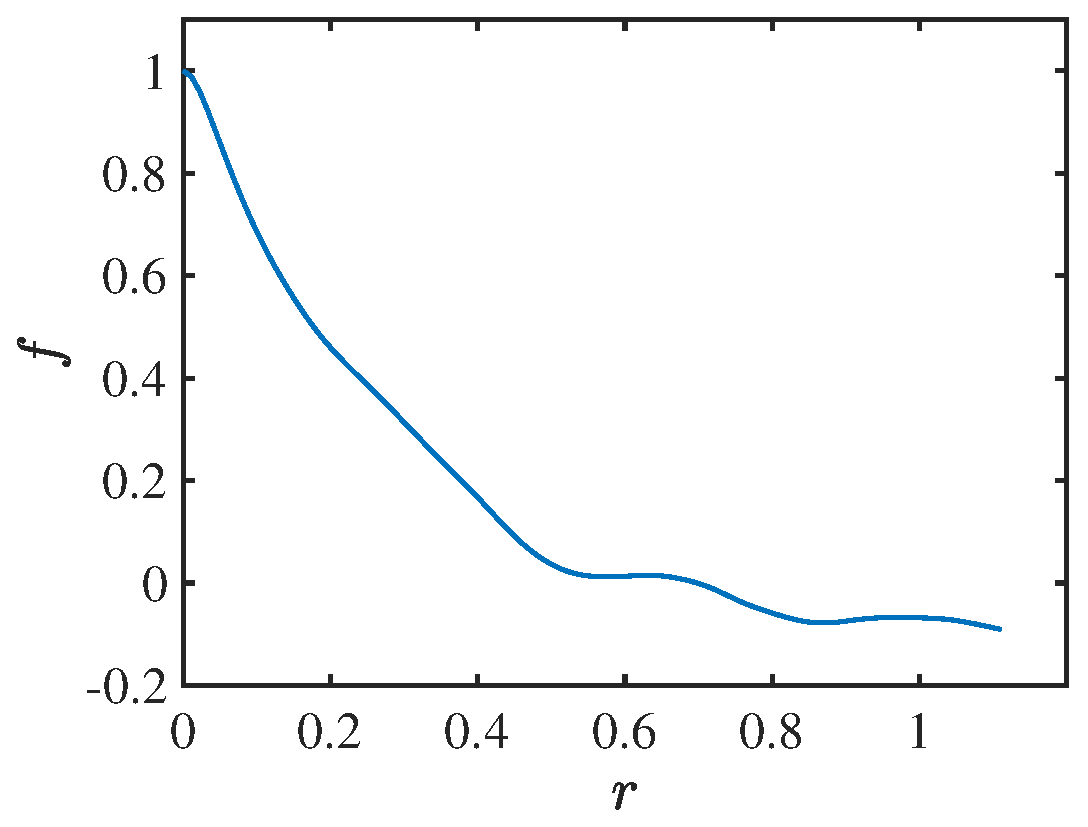
\includegraphics[width=.45\textwidth]{f-r.eps}}\quad
   \subfigure[三元速度关联函数$k$.]{\label{fig:k-r}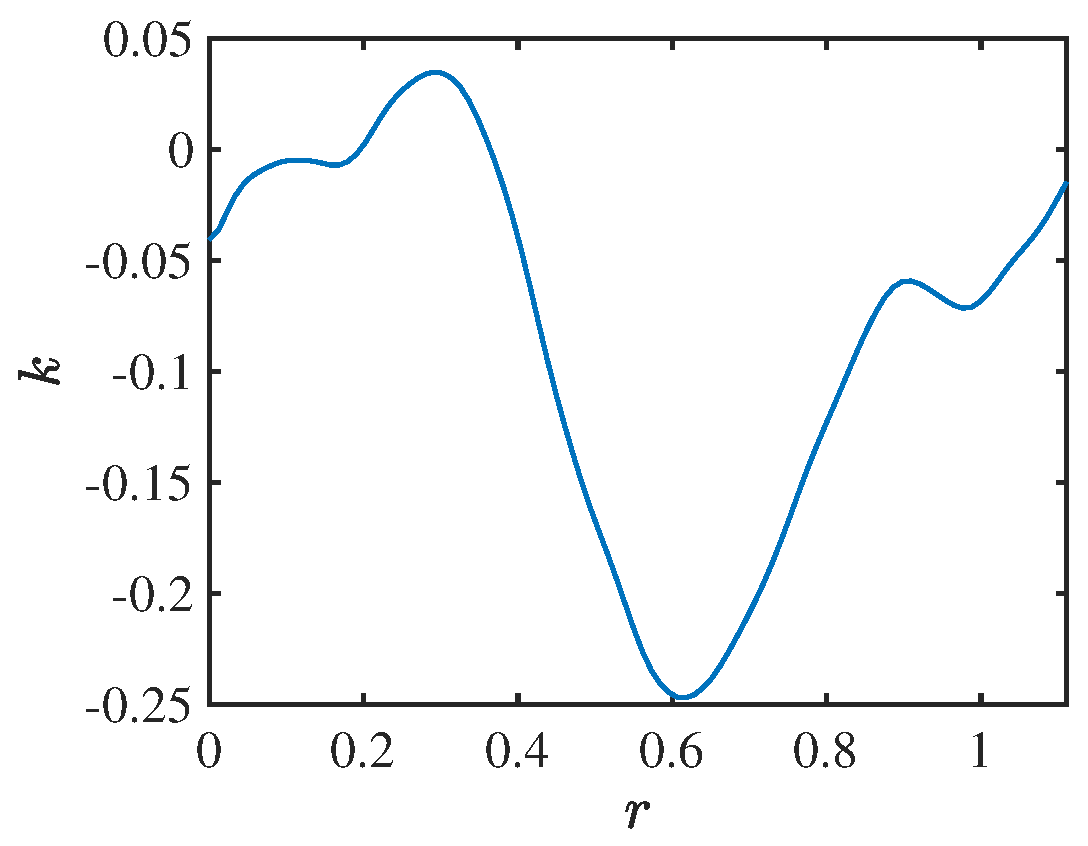
\includegraphics[width=.45\textwidth]{k-r.eps}}
   \caption{近似均匀各向同性同性湍流中的关联函数。}
   % \label{fig:Nu-k}
\end{figure}
三维能谱$E(k)$ 和$f(r)$ 的关系是
\begin{equation}
   E(k) = \frac{1}{\pi} \int_{0}^{+\infty} \left< u^2 \right> f(r) (kr)^{2} \left( \frac{\sin kr}{kr} - \cos kr \right) \dif r.
\end{equation}
一维能谱$\varphi(k)$ 和$E(k)$ 的关系是
\begin{equation}
   \varphi_1(k_1) = \frac{1}{2} \int_{k_1}^{+\infty} \left( 1 - \frac{k_1^2}{k^2} \frac{E(k)}{k}\right) \dif k.
\end{equation}
画图可得\cref{fig:E-k,fig:phi-k}.
\begin{figure}
   \centering
   \subfigure[三维能谱$E(k)$. ]{\label{fig:E-k}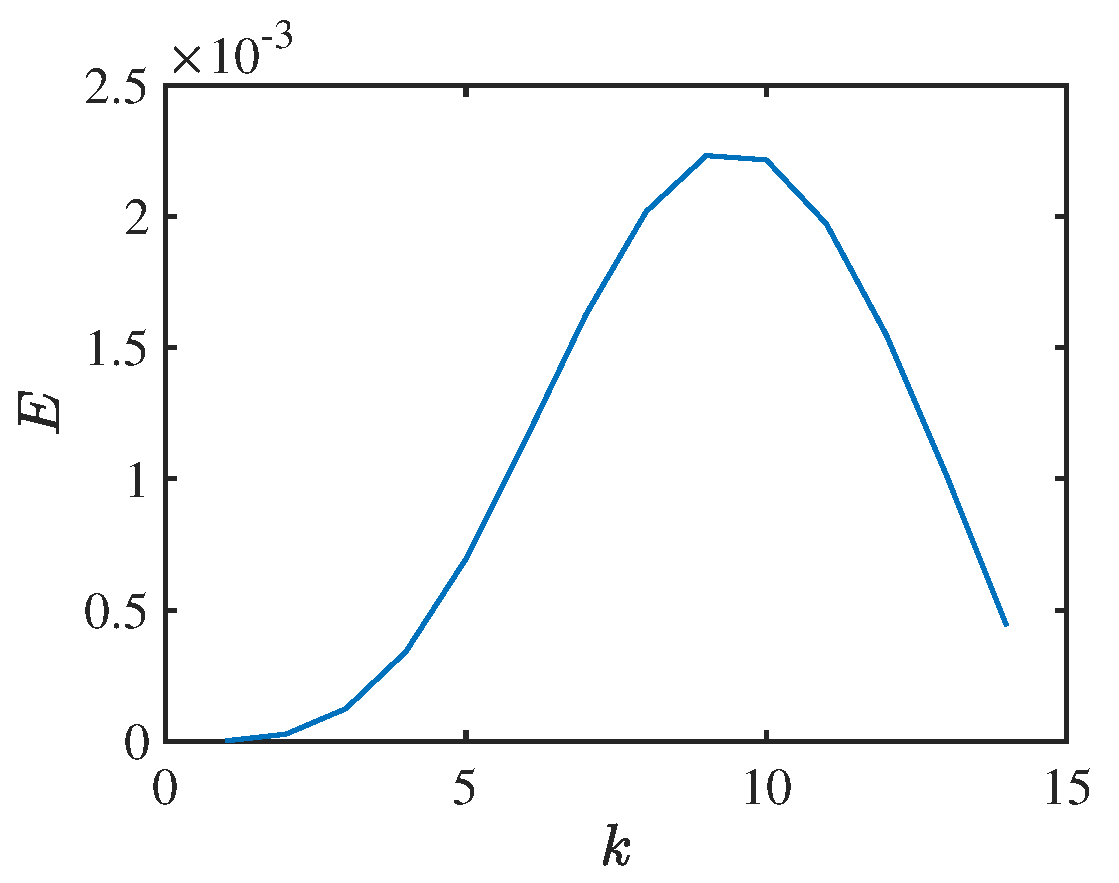
\includegraphics[width=.45\textwidth]{E-k.eps}}\quad
   \subfigure[一维能谱$\varphi(k)$.]{\label{fig:phi-k}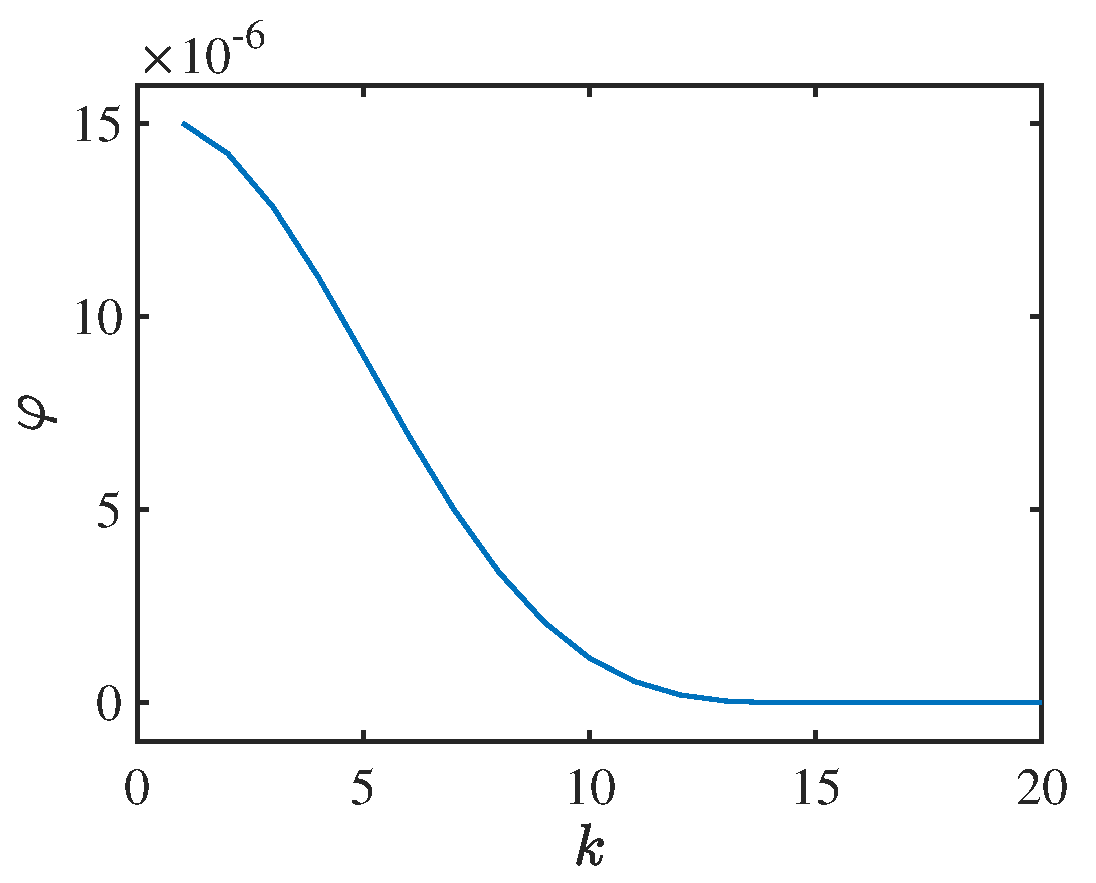
\includegraphics[width=.45\textwidth]{phi-k.eps}}
   \caption{能谱图。}
   % \label{fig:Nu-k}
\end{figure}












% \nocite{*}

% \newpage
\bibliographystyle{plain}
% \clearpage
\phantomsection

\addcontentsline{toc}{section}{参考文献} %向目录中添加条目,以章的名义
\bibliography{homework}

\end{document}
